% Options for packages loaded elsewhere
% Options for packages loaded elsewhere
\PassOptionsToPackage{unicode}{hyperref}
\PassOptionsToPackage{hyphens}{url}
%
\documentclass[
  11pt,
  ignorenonframetext,
  aspectratio=169,
]{beamer}
\newif\ifbibliography
\usepackage{pgfpages}
\setbeamertemplate{caption}[numbered]
\setbeamertemplate{caption label separator}{: }
\setbeamercolor{caption name}{fg=normal text.fg}
\beamertemplatenavigationsymbolsempty
% remove section numbering
\setbeamertemplate{part page}{
  \centering
  \begin{beamercolorbox}[sep=16pt,center]{part title}
    \usebeamerfont{part title}\insertpart\par
  \end{beamercolorbox}
}
\setbeamertemplate{section page}{
  \centering
  \begin{beamercolorbox}[sep=12pt,center]{section title}
    \usebeamerfont{section title}\insertsection\par
  \end{beamercolorbox}
}
\setbeamertemplate{subsection page}{
  \centering
  \begin{beamercolorbox}[sep=8pt,center]{subsection title}
    \usebeamerfont{subsection title}\insertsubsection\par
  \end{beamercolorbox}
}
% Prevent slide breaks in the middle of a paragraph
\widowpenalties 1 10000
\raggedbottom
\AtBeginPart{
  \frame{\partpage}
}
\AtBeginSection{
  \ifbibliography
  \else
    \frame{\sectionpage}
  \fi
}
\AtBeginSubsection{
  \frame{\subsectionpage}
}
\usepackage{iftex}
\ifPDFTeX
  \usepackage[T1]{fontenc}
  \usepackage[utf8]{inputenc}
  \usepackage{textcomp} % provide euro and other symbols
\else % if luatex or xetex
  \usepackage{unicode-math} % this also loads fontspec
  \defaultfontfeatures{Scale=MatchLowercase}
  \defaultfontfeatures[\rmfamily]{Ligatures=TeX,Scale=1}
\fi
\usepackage{lmodern}

\ifPDFTeX\else
  % xetex/luatex font selection
\fi
% Use upquote if available, for straight quotes in verbatim environments
\IfFileExists{upquote.sty}{\usepackage{upquote}}{}
\IfFileExists{microtype.sty}{% use microtype if available
  \usepackage[]{microtype}
  \UseMicrotypeSet[protrusion]{basicmath} % disable protrusion for tt fonts
}{}
\makeatletter
\@ifundefined{KOMAClassName}{% if non-KOMA class
  \IfFileExists{parskip.sty}{%
    \usepackage{parskip}
  }{% else
    \setlength{\parindent}{0pt}
    \setlength{\parskip}{6pt plus 2pt minus 1pt}}
}{% if KOMA class
  \KOMAoptions{parskip=half}}
\makeatother

\usepackage{color}
\usepackage{fancyvrb}
\newcommand{\VerbBar}{|}
\newcommand{\VERB}{\Verb[commandchars=\\\{\}]}
\DefineVerbatimEnvironment{Highlighting}{Verbatim}{commandchars=\\\{\}}
% Add ',fontsize=\small' for more characters per line
\usepackage{framed}
\definecolor{shadecolor}{RGB}{241,243,245}
\newenvironment{Shaded}{\begin{snugshade}}{\end{snugshade}}
\newcommand{\AlertTok}[1]{\textcolor[rgb]{0.68,0.00,0.00}{#1}}
\newcommand{\AnnotationTok}[1]{\textcolor[rgb]{0.37,0.37,0.37}{#1}}
\newcommand{\AttributeTok}[1]{\textcolor[rgb]{0.40,0.45,0.13}{#1}}
\newcommand{\BaseNTok}[1]{\textcolor[rgb]{0.68,0.00,0.00}{#1}}
\newcommand{\BuiltInTok}[1]{\textcolor[rgb]{0.00,0.23,0.31}{#1}}
\newcommand{\CharTok}[1]{\textcolor[rgb]{0.13,0.47,0.30}{#1}}
\newcommand{\CommentTok}[1]{\textcolor[rgb]{0.37,0.37,0.37}{#1}}
\newcommand{\CommentVarTok}[1]{\textcolor[rgb]{0.37,0.37,0.37}{\textit{#1}}}
\newcommand{\ConstantTok}[1]{\textcolor[rgb]{0.56,0.35,0.01}{#1}}
\newcommand{\ControlFlowTok}[1]{\textcolor[rgb]{0.00,0.23,0.31}{\textbf{#1}}}
\newcommand{\DataTypeTok}[1]{\textcolor[rgb]{0.68,0.00,0.00}{#1}}
\newcommand{\DecValTok}[1]{\textcolor[rgb]{0.68,0.00,0.00}{#1}}
\newcommand{\DocumentationTok}[1]{\textcolor[rgb]{0.37,0.37,0.37}{\textit{#1}}}
\newcommand{\ErrorTok}[1]{\textcolor[rgb]{0.68,0.00,0.00}{#1}}
\newcommand{\ExtensionTok}[1]{\textcolor[rgb]{0.00,0.23,0.31}{#1}}
\newcommand{\FloatTok}[1]{\textcolor[rgb]{0.68,0.00,0.00}{#1}}
\newcommand{\FunctionTok}[1]{\textcolor[rgb]{0.28,0.35,0.67}{#1}}
\newcommand{\ImportTok}[1]{\textcolor[rgb]{0.00,0.46,0.62}{#1}}
\newcommand{\InformationTok}[1]{\textcolor[rgb]{0.37,0.37,0.37}{#1}}
\newcommand{\KeywordTok}[1]{\textcolor[rgb]{0.00,0.23,0.31}{\textbf{#1}}}
\newcommand{\NormalTok}[1]{\textcolor[rgb]{0.00,0.23,0.31}{#1}}
\newcommand{\OperatorTok}[1]{\textcolor[rgb]{0.37,0.37,0.37}{#1}}
\newcommand{\OtherTok}[1]{\textcolor[rgb]{0.00,0.23,0.31}{#1}}
\newcommand{\PreprocessorTok}[1]{\textcolor[rgb]{0.68,0.00,0.00}{#1}}
\newcommand{\RegionMarkerTok}[1]{\textcolor[rgb]{0.00,0.23,0.31}{#1}}
\newcommand{\SpecialCharTok}[1]{\textcolor[rgb]{0.37,0.37,0.37}{#1}}
\newcommand{\SpecialStringTok}[1]{\textcolor[rgb]{0.13,0.47,0.30}{#1}}
\newcommand{\StringTok}[1]{\textcolor[rgb]{0.13,0.47,0.30}{#1}}
\newcommand{\VariableTok}[1]{\textcolor[rgb]{0.07,0.07,0.07}{#1}}
\newcommand{\VerbatimStringTok}[1]{\textcolor[rgb]{0.13,0.47,0.30}{#1}}
\newcommand{\WarningTok}[1]{\textcolor[rgb]{0.37,0.37,0.37}{\textit{#1}}}

\usepackage{longtable,booktabs,array}
\newcounter{none} % for unnumbered tables
\usepackage{calc} % for calculating minipage widths
\usepackage{caption}
% Make caption package work with longtable
\makeatletter
\def\fnum@table{\tablename~\thetable}
\makeatother
\usepackage{graphicx}
\makeatletter
\newsavebox\pandoc@box
\newcommand*\pandocbounded[1]{% scales image to fit in text height/width
  \sbox\pandoc@box{#1}%
  \Gscale@div\@tempa{\textheight}{\dimexpr\ht\pandoc@box+\dp\pandoc@box\relax}%
  \Gscale@div\@tempb{\linewidth}{\wd\pandoc@box}%
  \ifdim\@tempb\p@<\@tempa\p@\let\@tempa\@tempb\fi% select the smaller of both
  \ifdim\@tempa\p@<\p@\scalebox{\@tempa}{\usebox\pandoc@box}%
  \else\usebox{\pandoc@box}%
  \fi%
}
% Set default figure placement to htbp
\def\fps@figure{htbp}
\makeatother





\setlength{\emergencystretch}{3em} % prevent overfull lines

\providecommand{\tightlist}{%
  \setlength{\itemsep}{0pt}\setlength{\parskip}{0pt}}



 


\setbeamertemplate{navigation symbols}{}
\setbeamertemplate{footline}[frame number]
\setbeamertemplate{itemize items}[circle]
\setbeamertemplate{itemize subitem}[triangle]
\setbeamercolor{frametitle}{fg=black}
\setbeamerfont{frametitle}{series=\bfseries}
\newcommand{\indep}{\perp\!\!\!\perp}
\usepackage{booktabs}
\usepackage{tikz}
\usetikzlibrary{arrows.meta,positioning,calc}
\tikzset{
  dnode/.style={circle,draw,thick,minimum size=9mm,inner sep=1pt,font=\small},
  unode/.style={circle,draw,thick,dashed,minimum size=9mm,inner sep=1pt,font=\small},
  qnode/.style={circle,draw,thick,dotted,minimum size=9mm,inner sep=1pt,font=\small},
  de/.style={-{Stealth[length=2.2mm]},thick},
  dde/.style={-{Stealth[length=2.2mm]},thick,dashed}
}
\usepackage{fancyvrb}
\fvset{fontsize=\scriptsize}
\makeatletter
\def\verbatim@font{\scriptsize\ttfamily}
\makeatother
\makeatletter
\@ifpackageloaded{caption}{}{\usepackage{caption}}
\AtBeginDocument{%
\ifdefined\contentsname
  \renewcommand*\contentsname{Table of contents}
\else
  \newcommand\contentsname{Table of contents}
\fi
\ifdefined\listfigurename
  \renewcommand*\listfigurename{List of Figures}
\else
  \newcommand\listfigurename{List of Figures}
\fi
\ifdefined\listtablename
  \renewcommand*\listtablename{List of Tables}
\else
  \newcommand\listtablename{List of Tables}
\fi
\ifdefined\figurename
  \renewcommand*\figurename{Figure}
\else
  \newcommand\figurename{Figure}
\fi
\ifdefined\tablename
  \renewcommand*\tablename{Table}
\else
  \newcommand\tablename{Table}
\fi
}
\@ifpackageloaded{float}{}{\usepackage{float}}
\floatstyle{ruled}
\@ifundefined{c@chapter}{\newfloat{codelisting}{h}{lop}}{\newfloat{codelisting}{h}{lop}[chapter]}
\floatname{codelisting}{Listing}
\newcommand*\listoflistings{\listof{codelisting}{List of Listings}}
\makeatother
\makeatletter
\makeatother
\makeatletter
\@ifpackageloaded{caption}{}{\usepackage{caption}}
\@ifpackageloaded{subcaption}{}{\usepackage{subcaption}}
\makeatother

\usepackage{bookmark}
\IfFileExists{xurl.sty}{\usepackage{xurl}}{} % add URL line breaks if available
\urlstyle{same}
\hypersetup{
  pdftitle={Instrumental Variables},
  pdfauthor={Professor Ji-Woong Chung},
  hidelinks,
  pdfcreator={LaTeX via pandoc}}


\title{\texorpdfstring{Instrumental Variables}{Instrumental Variables}}
\subtitle{\texorpdfstring{BUSS975: Causal Inference in Financial
Research}{BUSS975: Causal Inference in Financial Research}}
\author{Professor Ji-Woong Chung}
\date{}
\institute{Korea University}

\begin{document}
\frame{\titlepage}


\section{7.1 The Strangeness Principle}\label{the-strangeness-principle}

\begin{frame}{Where we left off}
\protect\phantomsection\label{where-we-left-off}
\begin{itemize}
\tightlist
\item
  \textbf{Lecture 4 (RD).} Identification came from a \emph{rule}: a
  known threshold in a running variable. One assumption --- continuity
  --- and an estimand at one point.
\item
  \textbf{Today (IV).} Identification comes from a \emph{shock}:
  something in the world that pushes units into and out of treatment for
  reasons unrelated to their outcomes.
\item
  The problem IV addresses is the one matching and RD could not touch:
  \textbf{selection on unobservables}. You believe \(D\) is correlated
  with something you cannot measure, and no amount of conditioning will
  fix it.
\item
  The price is steep. RD has one main identifying assumption. IV, under
  heterogeneous effects, has \textbf{five} --- and the most important
  one is untestable.
\item
  Cunningham's framing: IV is ``unfairly maligned, poorly understood,
  very hard to imitate well.'' Finding a valid instrument is like
  finding a four-leaf clover.
\end{itemize}
\end{frame}

\begin{frame}{A strange thing happened at Thanksgiving}
\protect\phantomsection\label{a-strange-thing-happened-at-thanksgiving}
\begin{itemize}
\tightlist
\item
  Your brother, four years into a PhD, produces a chart at dinner.
  Mothers whose \textbf{first two children are the same sex} --- two
  boys or two girls --- are about \textbf{one percentage point less
  likely} to work for pay than mothers whose first two are a boy and a
  girl.
\item
  Everyone at the table stares. Why on earth would the \emph{sexes} of
  two children have anything to do with whether their mother holds a
  job? Two boys are no more burdensome than one of each.
\item
  Nobody can explain it. That baffled reaction is the point.
\item
  This is a real result: \textbf{Angrist and Evans (1998)}.
\end{itemize}

\vspace{0.4em}

\begin{itemize}
\tightlist
\item
  The DAG you are implicitly drawing has a \textbf{hole} in it.
\end{itemize}
\end{frame}

\begin{frame}{The hole in the DAG}
\protect\phantomsection\label{the-hole-in-the-dag}
\begin{center}
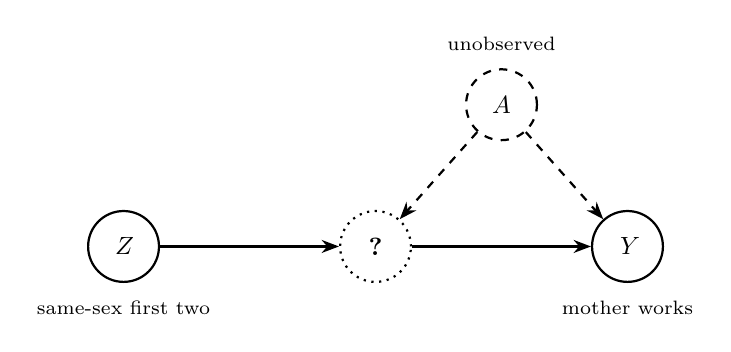
\begin{tikzpicture}[node distance=22mm]
\node[dnode] (Z) at (0,0) {$Z$};
\node[qnode] (Q) at (3.2,0) {\textbf{?}};
\node[dnode] (Y) at (6.4,0) {$Y$};
\node[unode] (A) at (4.8,1.8) {$A$};
\draw[de] (Z) -- (Q);
\draw[de] (Q) -- (Y);
\draw[dde] (A) -- (Q);
\draw[dde] (A) -- (Y);
\node[below=1mm of Z, font=\scriptsize] {same-sex first two};
\node[below=1mm of Y, font=\scriptsize] {mother works};
\node[above=1mm of A, font=\scriptsize] {unobserved};
\end{tikzpicture}
\end{center}

\begin{itemize}
\tightlist
\item
  You know the instrument, the outcome, and maybe the confounders.
  \textbf{You do not know the treatment} --- and that missing link is
  the source of the strangeness.
\item
  Fill the hole with \textbf{family size} and it evaporates: parents who
  want a mix of sexes and get two of a kind try for a third child, and a
  third child changes labour supply.
\item
  Sex ratios are valid \emph{because} they move family size and are
  otherwise unrelated to the mother's labour supply.
\end{itemize}
\end{frame}

\begin{frame}{The strangeness principle}
\protect\phantomsection\label{the-strangeness-principle-1}
\begin{quote}
A valid instrument neither directly causes the outcome, nor is
correlated with anything else that does --- \textbf{except through the
treatment.}
\end{quote}

\begin{itemize}
\tightlist
\item
  Because the treatment is absent from the raw \(Z\)--\(Y\) correlation,
  any association you find \emph{should not be there}. The feeling of
  strangeness is the informal smell test that it is not.
\item
  \textbf{Aunt Linda.} She runs a celebrated restaurant. Asked how it
  started, she says: \emph{``Jury duty.''} You blink. Sequestered for
  three weeks, she helped the courthouse cook, who taught her
  everything; a year later they opened together.
\item
  Jury duty \(\to\) apprenticeship \(\to\) success. Once you learn about
  the apprenticeship, the strangeness disappears. Jury service has no
  direct path to culinary fame --- which is exactly what makes it a
  usable instrument.
\item
  Note what the strangeness is \emph{not}: it is not evidence. It is a
  prompt to go looking for the mechanism.
\end{itemize}
\end{frame}

\begin{frame}{When nothing feels strange, be suspicious}
\protect\phantomsection\label{when-nothing-feels-strange-be-suspicious}
\begin{center}
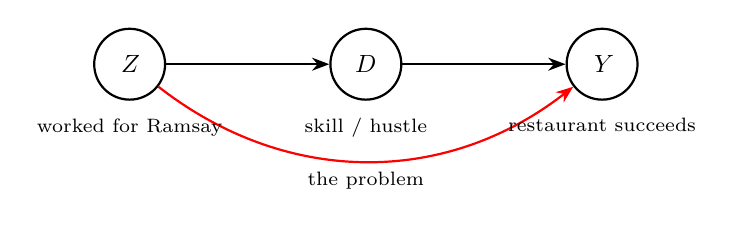
\begin{tikzpicture}[node distance=20mm]
\node[dnode] (Z) at (0,0) {$Z$};
\node[dnode] (D) at (3.0,0) {$D$};
\node[dnode] (Y) at (6.0,0) {$Y$};
\draw[de] (Z) -- (D);
\draw[de] (D) -- (Y);
\draw[de,red,thick] (Z) to[bend right=38] node[below,font=\scriptsize,midway,black] {the problem} (Y);
\node[below=1mm of Z, font=\scriptsize] {worked for Ramsay};
\node[below=1mm of D, font=\scriptsize] {skill / hustle};
\node[below=1mm of Y, font=\scriptsize] {restaurant succeeds};
\end{tikzpicture}
\end{center}

\begin{itemize}
\tightlist
\item
  Cousin Jacob also became a chef. He was a line cook on one of
  \textbf{Gordon Ramsay's} shows, and credits his own hustle for
  everything since.
\item
  The table laughs. There is \textbf{nothing strange} about someone who
  worked with Ramsay going on to succeed --- his name alone brings
  investors, press, partnerships and early customers.
\item
  That red arrow is a direct path from instrument to outcome. It is a
  violation of the \textbf{exclusion restriction}, and it cannot be
  fixed by any estimator.
\item
  \textbf{The diagnostic:} if an intelligent layperson hears your
  reduced form and nods, you probably do not have an instrument. If they
  frown and ask ``why would \emph{those} two things be related?'', you
  might.
\end{itemize}
\end{frame}

\begin{frame}{Instruments are treatment assignment mechanisms}
\protect\phantomsection\label{instruments-are-treatment-assignment-mechanisms}
\begin{itemize}
\tightlist
\item
  The deeper claim, and the one worth carrying out of this lecture:
  \textbf{a valid instrument corresponds to something in the real world
  that literally moves units into and out of treatment.} Coin flips.
  Draft numbers. Lotteries. Weather.
\item
  IV does \textbf{not} create exogenous variation. That variation either
  exists in the world or it does not. The model cannot summon it --- it
  can only exploit it.
\item
  So the best instruments come from \textbf{institutional knowledge} of
  how the treatment is actually assigned, not from searching a dataset
  for something correlated with \(D\).
\item
  Cunningham's practical advice: talk to people. Ask them, in their own
  words, how some ended up treated and others did not. Do not ask them
  to name an instrument --- they have not read the book. Just listen.
\item
  You will notice this is the same discipline that §6.4 demanded of RD:
  \emph{know the rule}. Here: \emph{know the shock}.
\end{itemize}
\end{frame}

\section{7.2 The Wald Estimator}\label{the-wald-estimator}

\begin{frame}{When OLS is biased}
\protect\phantomsection\label{when-ols-is-biased}
\begin{center}
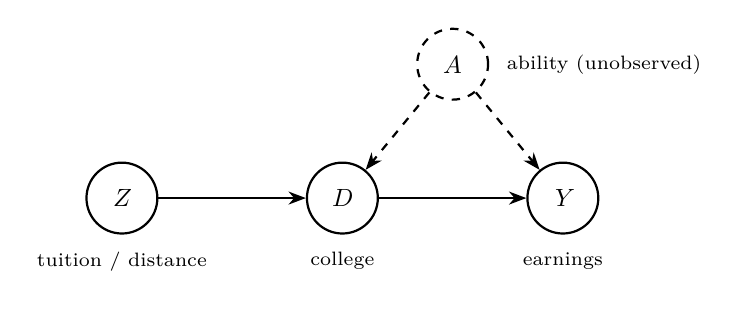
\begin{tikzpicture}[node distance=20mm]
\node[dnode] (Z) at (0,0) {$Z$};
\node[dnode] (D) at (2.8,0) {$D$};
\node[dnode] (Y) at (5.6,0) {$Y$};
\node[unode] (A) at (4.2,1.7) {$A$};
\draw[de] (Z) -- (D);
\draw[de] (D) -- (Y);
\draw[dde] (A) -- (D);
\draw[dde] (A) -- (Y);
\node[below=1mm of Z, font=\scriptsize] {tuition / distance};
\node[below=1mm of D, font=\scriptsize] {college};
\node[below=1mm of Y, font=\scriptsize] {earnings};
\node[right=1mm of A, font=\scriptsize] {ability (unobserved)};
\end{tikzpicture}
\end{center}

Suppose the true model of earnings is \[
Y_i = \alpha + \delta D_i + \gamma A_i + \varepsilon_i,
\] but \(A\) is not in your data, so you estimate
\(Y_i = \alpha + \delta D_i + \eta_i\) with
\(\eta_i = \gamma A_i + \varepsilon_i\).

\begin{itemize}
\tightlist
\item
  \textbf{The question for this section:} what does OLS on the short
  regression actually give you?
\end{itemize}
\end{frame}

\begin{frame}{The omitted variable bias formula}
\protect\phantomsection\label{the-omitted-variable-bias-formula}
Write \(C(\cdot,\cdot)\) for covariance and \(V(\cdot)\) for variance.
OLS is a scaled covariance: \[
\hat\delta = \frac{C(Y, D)}{V(D)}.
\] Substitute the \emph{long} model for \(Y\) and expand: \[
\begin{aligned}
\hat\delta
&= \frac{\delta V(D) + \gamma\,C(D,A) + C(D,\varepsilon)}{V(D)} \\[0.3em]
&= \delta \;+\; \gamma\,\frac{C(A,D)}{V(D)}
\qquad\text{since } C(D,\varepsilon) = 0 .
\end{aligned}
\]

\begin{itemize}
\tightlist
\item
  The second term is the bias. If ability raises earnings
  (\(\gamma > 0\)) and the able get more schooling (\(C(A,D) > 0\)), OLS
  is \textbf{biased upward}.
\item
  Nothing about this is fixed by more data: the bias does not shrink
  with \(n\). It is a property of the population, not the sample.
\item
  You cannot condition your way out, because \(A\) is unobserved. That
  is the whole problem.
\end{itemize}
\end{frame}

\begin{frame}{The trick: take the covariance with \(Z\) instead}
\protect\phantomsection\label{the-trick-take-the-covariance-with-z-instead}
Keep the long model and compute \(C(Y,Z)\) rather than \(C(Y,D)\): \[
C(Y,Z) \;=\; \delta\,C(D,Z) \;+\; \gamma\,C(A,Z) \;+\; C(\varepsilon,Z).
\]

\begin{itemize}
\tightlist
\item
  In the DAG, there is no open path from \(Z\) to \(A\): every route
  runs through a \textbf{collider} (\(Z \to D \leftarrow A\), and
  \(Z \to D \to Y \leftarrow A\)). So \(C(A,Z) = 0\). Likewise
  \(C(\varepsilon, Z) = 0\).
\item
  Both of the troublesome terms vanish: \[
  C(Y,Z) = \delta\,C(D,Z).
  \]
\item
  It is a free country, so divide both sides by \(C(D,Z)\): \[
  \boxed{\;\hat\delta_{\text{Wald}} \;=\; \frac{C(Y,Z)}{C(D,Z)} \;=\; \delta\;}
  \]
\item
  Two covariances. You could compute them with a pencil and a
  spreadsheet.
\end{itemize}
\end{frame}

\begin{frame}{Reduced form and first stage}
\protect\phantomsection\label{reduced-form-and-first-stage}
\[
\underbrace{\frac{C(Y,Z)}{C(D,Z)}}_{\textstyle \hat\delta_{\text{Wald}}}
\qquad=\qquad
\frac{\text{\textbf{Reduced form}}}{\text{\textbf{First stage}}}
\]

\begin{itemize}
\tightlist
\item
  The \textbf{reduced form}, \(C(Y,Z)\), is the strange association
  itself --- the \(Z\)--\(Y\) correlation that should not be there.
  Angrist--Evans: sex ratios and maternal labour supply.
\item
  The \textbf{first stage}, \(C(D,Z)\), is the association between
  instrument and treatment. It is what \emph{resolves} the strangeness.
\item
  You will hear this jargon constantly from now on. Learn it here.
\item
  \textbf{A nontrivial point.} The reduced form is \emph{just a
  calculation}. It can always be computed, and computing it tells you
  nothing about whether the instrument is valid. Keep ``I can compute
  it'' and ``it identifies something'' firmly apart.
\end{itemize}
\end{frame}

\begin{frame}{What makes it work, and what cannot be checked}
\protect\phantomsection\label{what-makes-it-work-and-what-cannot-be-checked}
The Wald estimator recovers \(\delta\) when:

\begin{enumerate}
\tightlist
\item
  \textbf{Exclusion.} \(Z\) does not cause \(Y\) directly --- any effect
  runs through \(D\).
\item
  \textbf{Independence.} \(Z\) is independent of the confounder \(A\)
  and the error \(\varepsilon\).
\item
  \textbf{A nonzero first stage.} \(C(D,Z) \neq 0\).
\end{enumerate}

\vspace{0.4em}

\begin{itemize}
\tightlist
\item
  Under these, \(\operatorname{plim} \hat\delta = \delta\):
  \textbf{consistency}. In finite samples it differs, and by how much
  depends largely on the strength of that denominator --- §7.4.
\item
  \textbf{The bad news.} Exclusion cannot be tested, at least not
  without extra assumptions you will not like. Arguments for it are
  \emph{narrative}.
\item
  Good narratives rest on a realistic understanding of how treatment is
  actually assigned --- shoe-leather, not data mining. Bad ones rest on
  the word ``exogenous.''
\item
  This is why IV attracts scepticism: defeating an IV paper requires
  only creating doubt about exclusion.
\end{itemize}
\end{frame}

\section{7.3 Two Stage Least Squares}\label{two-stage-least-squares}

\begin{frame}{Wald \emph{is} 2SLS}
\protect\phantomsection\label{wald-is-2sls}
Start from the Wald ratio and multiply through by \(V(Z)/V(Z)\): \[
\hat\delta_{\text{Wald}}
= \frac{C(Z,Y)}{C(Z,D)}
= \frac{C(Z,Y)/V(Z)}{C(Z,D)/V(Z)}
= \frac{\hat\beta\,C(Z,Y)}{\hat\beta^{2} V(Z)}
= \frac{C(\hat\beta Z, Y)}{V(\hat\beta Z)},
\] where \(\hat\beta = C(Z,D)/V(Z)\) is the first-stage slope from
\(D = \gamma + \beta Z + \epsilon\).

\begin{itemize}
\tightlist
\item
  But \(\hat\beta Z\) is, up to the constant, the \textbf{fitted value}
  \(\hat D\) from that first stage. So \[
  \hat\delta_{2SLS} = \frac{C(\hat D, Y)}{V(\hat D)} .
  \]
\item
  We are no longer using \(D\). We are using the part of \(D\) that the
  instrument explains --- the part that is, by assumption, unrelated to
  \(A\).
\item
  \textbf{Without covariates, Wald and 2SLS are numerically identical.}
  Not approximately. Identically.
\end{itemize}
\end{frame}

\begin{frame}[fragile]{Four ways, one number}
\protect\phantomsection\label{four-ways-one-number}
\begin{Shaded}
\begin{Highlighting}[]
\FunctionTok{suppressMessages}\NormalTok{(\{}\FunctionTok{library}\NormalTok{(haven); }\FunctionTok{library}\NormalTok{(AER)\})}
\NormalTok{card }\OtherTok{\textless{}{-}} \FunctionTok{as.data.frame}\NormalTok{(}\FunctionTok{read\_dta}\NormalTok{(}\StringTok{"data/card.dta"}\NormalTok{))}
\NormalTok{d }\OtherTok{\textless{}{-}}\NormalTok{ card[}\SpecialCharTok{!}\FunctionTok{is.na}\NormalTok{(card}\SpecialCharTok{$}\NormalTok{lwage) }\SpecialCharTok{\&} \SpecialCharTok{!}\FunctionTok{is.na}\NormalTok{(card}\SpecialCharTok{$}\NormalTok{educ) }\SpecialCharTok{\&} \SpecialCharTok{!}\FunctionTok{is.na}\NormalTok{(card}\SpecialCharTok{$}\NormalTok{nearc4), ]}

\NormalTok{w1 }\OtherTok{\textless{}{-}} \FunctionTok{cov}\NormalTok{(d}\SpecialCharTok{$}\NormalTok{lwage, d}\SpecialCharTok{$}\NormalTok{nearc4) }\SpecialCharTok{/} \FunctionTok{cov}\NormalTok{(d}\SpecialCharTok{$}\NormalTok{educ, d}\SpecialCharTok{$}\NormalTok{nearc4)        }\CommentTok{\# ratio of covariances}
\NormalTok{w2 }\OtherTok{\textless{}{-}} \FunctionTok{coef}\NormalTok{(}\FunctionTok{lm}\NormalTok{(lwage }\SpecialCharTok{\textasciitilde{}}\NormalTok{ nearc4, d))[}\DecValTok{2}\NormalTok{] }\SpecialCharTok{/} \FunctionTok{coef}\NormalTok{(}\FunctionTok{lm}\NormalTok{(educ }\SpecialCharTok{\textasciitilde{}}\NormalTok{ nearc4, d))[}\DecValTok{2}\NormalTok{]  }\CommentTok{\# ratio of OLS}
\NormalTok{fs }\OtherTok{\textless{}{-}} \FunctionTok{lm}\NormalTok{(educ }\SpecialCharTok{\textasciitilde{}}\NormalTok{ nearc4, d)}
\NormalTok{w3 }\OtherTok{\textless{}{-}} \FunctionTok{coef}\NormalTok{(}\FunctionTok{lm}\NormalTok{(d}\SpecialCharTok{$}\NormalTok{lwage }\SpecialCharTok{\textasciitilde{}} \FunctionTok{fitted}\NormalTok{(fs)))[}\DecValTok{2}\NormalTok{]                     }\CommentTok{\# manual two stages}
\NormalTok{w4 }\OtherTok{\textless{}{-}} \FunctionTok{coef}\NormalTok{(}\FunctionTok{ivreg}\NormalTok{(lwage }\SpecialCharTok{\textasciitilde{}}\NormalTok{ educ }\SpecialCharTok{|}\NormalTok{ nearc4, }\AttributeTok{data =}\NormalTok{ d))[}\DecValTok{2}\NormalTok{]       }\CommentTok{\# one command}
\FunctionTok{setNames}\NormalTok{(}\FunctionTok{unname}\NormalTok{(}\FunctionTok{c}\NormalTok{(w1, w2, w3, w4)),}
         \FunctionTok{c}\NormalTok{(}\StringTok{"covariances"}\NormalTok{, }\StringTok{"OLS ratio"}\NormalTok{, }\StringTok{"manual 2SLS"}\NormalTok{, }\StringTok{"ivreg"}\NormalTok{))}
\end{Highlighting}
\end{Shaded}

\begin{verbatim}
covariances   OLS ratio manual 2SLS       ivreg 
  0.1880626   0.1880626   0.1880626   0.1880626 
\end{verbatim}

\footnotesize

Card (1995), \(N = 3{,}010\). Identical to the last digit, because they
are the same estimator written four ways. Compare OLS on the same data:
0.0521.
\end{frame}

\begin{frame}[fragile]{One warning about doing it by hand}
\protect\phantomsection\label{one-warning-about-doing-it-by-hand}
\begin{itemize}
\tightlist
\item
  You may compute 2SLS in two manual steps to \textbf{see} what it does.
  Never \emph{report} results that way.
\item
  The second-stage standard errors from a manual two-step regression are
  \textbf{wrong}. They treat \(\hat D\) as if it were data, ignoring
  that it was estimated --- so they are too small.
\item
  Use \texttt{ivreg} (R, \texttt{AER} or \texttt{ivreg} package) or
  \texttt{ivregress\ 2sls} (Stata), which compute the correct variance.
\item
  With covariates \(X\), the rule is: \textbf{every exogenous regressor
  is its own instrument.} \(X\) appears in both stages; only \(D\) is
  instrumented.
\item
  With more instruments than endogenous regressors the model is
  \textbf{over-identified}, and 2SLS uses a particular weighted
  combination of them. That is where §7.4's trouble begins.
\end{itemize}
\end{frame}

\section{7.4 Weak Instruments}\label{weak-instruments}

\begin{frame}{Quarter of birth and compulsory schooling}
\protect\phantomsection\label{quarter-of-birth-and-compulsory-schooling}
\begin{itemize}
\tightlist
\item
  \textbf{Angrist and Krueger (1991).} Two institutional facts,
  combined:

  \begin{enumerate}
  \tightlist
  \item
    Children start first grade based on a \textbf{31 December} cutoff.
    Two children born a day apart, 31 December and 1 January, start a
    year apart --- purely by chance.
  \item
    Compulsory schooling laws let students leave at \textbf{16}.
  \end{enumerate}
\item
  A child born in the fourth quarter therefore reaches 16 having
  completed \emph{more} schooling than one born in the first quarter.
  The law binds them differently through nothing but their birthday.
\item
  So quarter of birth shifts years of schooling --- a little, for some
  people --- and is otherwise, one hopes, unrelated to earnings.
\item
  \textbf{The strangeness test:} tell someone that people born in
  January earn less than people born in October. They will frown. Good.
\end{itemize}
\end{frame}

\begin{frame}{Present the Wald estimator as two pictures}
\protect\phantomsection\label{present-the-wald-estimator-as-two-pictures}
\begin{itemize}
\tightlist
\item
  Angrist and Krueger show the \textbf{first stage} --- years of
  schooling by quarter of birth, cohort by cohort --- as a figure, not a
  coefficient. Fourth- and third-quarter births sit visibly higher.
\item
  They show the \textbf{reduced form} --- log weekly earnings by quarter
  of birth --- the same way. Jagged, but the 3s and 4s sit above the 1s
  and 2s.
\item
  Those two figures \emph{are} the numerator and the denominator of the
  Wald estimator. The paper shows you the estimate before it ever runs
  2SLS.
\item
  \textbf{The rule for your own work:} visualise the reduced form and
  the first stage separately, even if you will ultimately report 2SLS. A
  plot of \(Y\) against \(\hat D\) is opaque and invites suspicion,
  because the data have already been processed.
\item
  A second thing the figure reveals: the relationship \textbf{fades for
  later cohorts}. By the 1947 births it has nearly vanished. Hold that
  thought.
\end{itemize}
\end{frame}

\begin{frame}{A falsification test built into the first stage}
\protect\phantomsection\label{a-falsification-test-built-into-the-first-stage}
\begin{center}
\small
\begin{tabular}{llrrr}
\toprule
Outcome & Cohort & QOB I & QOB II & QOB III \\
\midrule
Total schooling  & 1930--39 & $-0.124$ & $-0.086$ & $-0.015$ \\
High school grad & 1930--39 & $-0.019$ & $-0.020$ & $-0.004$ \\
\textbf{College grad} & 1930--39 & $-0.005$ & $\phantom{-}0.003$ & $\phantom{-}0.002$ \\
\bottomrule
\end{tabular}
\end{center}

\begin{itemize}
\tightlist
\item
  Quarter of birth predicts \textbf{total schooling} and \textbf{high
  school graduation}, both negative and significant: born earlier in the
  year, less schooling. That is the first stage.
\item
  It does \textbf{not} predict \textbf{college graduation}. And that is
  the point.
\item
  Compulsory schooling binds only through high school. If quarter of
  birth predicted college completion, postgraduate degrees and total
  years alike, the instrument would clearly be picking up something
  \emph{other} than the compulsory-schooling channel --- and exclusion
  would be in doubt.
\item
  \textbf{The general lesson.} Where your proposed mechanism implies the
  instrument should have \emph{no} effect, show that it has no effect.
  Untestable assumptions have testable implications; go find them.
\end{itemize}
\end{frame}

\begin{frame}{More instruments, more precision --- at what price?}
\protect\phantomsection\label{more-instruments-more-precision-at-what-price}
\begin{itemize}
\tightlist
\item
  Angrist and Krueger wanted more variation in predicted schooling,
  which should mean more precision. So they interacted the three quarter
  dummies with state and year of birth: \textbf{180 instruments}.
\item
  At the time this looked like a free lunch. It was not.
\item
  Many of the extra instruments are \textbf{nearly useless}: in some
  states quarter of birth explains almost nothing, and in later cohorts
  the effect had faded (that figure again).
\item
  \textbf{Bound, Jaeger and Baker (1995)} showed what this does. Writing
  the OLS bias as \(\sigma_{\varepsilon\eta}/\sigma_\eta^2\), the
  finite-sample bias of 2SLS is approximately \[
  E[\hat\beta_{2SLS} - \beta] \;\approx\; \frac{\sigma_{\varepsilon\eta}}{\sigma_\eta^{2}} \cdot \frac{1}{F + 1},
  \] where \(F\) is the population first-stage \(F\)-statistic.
\item
  Read it: as \(F \to \infty\) the bias vanishes; as \(F \to 0\)
  \textbf{2SLS converges on the OLS bias}. Adding weak instruments
  lowers \(F\) and so moves you back toward the thing you were trying to
  escape.
\end{itemize}
\end{frame}

\begin{frame}{What weak instruments actually do}
\protect\phantomsection\label{what-weak-instruments-actually-do}
\pandocbounded{\includegraphics[keepaspectratio]{05_instrumental_variables_files/figure-beamer/unnamed-chunk-2-1.pdf}}

\vspace{-0.3em}
\footnotesize

True effect \(= 1\); OLS is biased to about \(1.8\). \textbf{Left:} as
the first stage weakens, median 2SLS slides off the truth and onto the
OLS bias --- and at the traditional threshold \(F = 10\) it is still
visibly biased. \textbf{Right:} \(K\) instruments that are \emph{pure
random noise}, containing no information about \(D\) whatsoever. The
estimates are tight, confident, and wrong.
\end{frame}

\begin{frame}{Krueger's own suggestion, and what it showed}
\protect\phantomsection\label{kruegers-own-suggestion-and-what-it-showed}
\begin{itemize}
\tightlist
\item
  Bound, Jaeger and Baker re-ran Angrist and Krueger's specifications
  using \textbf{randomly generated numbers} in place of actual quarter
  of birth. The idea was Alan Krueger's own.
\item
  Their finding, in their words: the second-stage results \emph{``look
  quite reasonable even with no information about educational attainment
  in the simulated instruments. They give no indication that the
  instruments were randomly generated.''}
\item
  But: \emph{``the F statistics on the excluded instruments in the
  first-stage regressions are always near their expected value of
  essentially 1 and do give a clear indication''} of the problem.
\item
  That is the right panel above, reproduced. \textbf{The second stage
  cannot warn you. Only the first stage can.}
\item
  In the real data, adding controls drove Angrist and Krueger's
  first-stage \(F\) from \(13.5\) to \(4.8\) to \(1.6\) --- and the 2SLS
  estimate drifted back toward OLS, exactly as the formula predicts.
\end{itemize}
\end{frame}

\begin{frame}{How should we measure weakness?}
\protect\phantomsection\label{how-should-we-measure-weakness}
\begin{itemize}
\tightlist
\item
  \textbf{The old rule.} Stock and Yogo (2005): first-stage \(F > 10\).
  Based on Monte Carlo under homoskedasticity. For twenty years this was
  the standard.
\item
  \textbf{The number 10 is now considered too low}, especially with
  multiple endogenous regressors, heteroskedasticity, or non-normal
  errors. Lee et al.~(2022) argue the relevant threshold can be above
  \textbf{100}.
\item
  Weak instruments do not merely bias point estimates. They
  \textbf{distort inference}: standard errors come out too small and
  \(t\)-tests mislead.
\item
  \textbf{What to report now}, following Andrews, Stock and Sun (2019):

  \begin{enumerate}
  \tightlist
  \item
    The \textbf{effective \(F\)-statistic} of Montiel Olea and Pflueger
    (2013), which accounts for heteroskedasticity. In the
    just-identified case it reduces to the robust first-stage \(F\).
  \item
    \textbf{Anderson--Rubin confidence intervals} --- \emph{regardless}
    of the value of \(F\).
  \end{enumerate}
\end{itemize}
\end{frame}

\begin{frame}{Anderson--Rubin intervals}
\protect\phantomsection\label{andersonrubin-intervals}
\begin{itemize}
\tightlist
\item
  A conventional 2SLS interval is built \textbf{around a point
  estimate}: \(\hat\delta \pm 1.96\,\widehat{SE}\). That construction
  presumes \(\hat\delta\) is well behaved, which under weak instruments
  it is not.
\item
  An AR interval instead \textbf{inverts a hypothesis test}. For each
  candidate value \(\delta_0\), it asks: could this value plausibly have
  generated the data? Values that could not are excluded.
\item
  The payoff: AR intervals are valid \textbf{whether or not the
  instrument is strong}.

  \begin{itemize}
  \tightlist
  \item
    Strong instrument \(\Rightarrow\) the interval is tight.
  \item
    Weak instrument \(\Rightarrow\) the interval expands, sometimes to
    include both large positive and large negative values.
  \end{itemize}
\item
  That blow-up is not a failure of the method. It is the method
  \textbf{telling you the truth}: your instrument is not strong enough
  to learn anything from these data.
\item
  With multiple instruments the literature has not converged on one
  procedure. Report a robust one, and say which.
\end{itemize}
\end{frame}

\begin{frame}{So what do you do with a weak instrument?}
\protect\phantomsection\label{so-what-do-you-do-with-a-weak-instrument}
\begin{itemize}
\tightlist
\item
  \textbf{Use a just-identified model with your single strongest
  instrument.} Fewer, stronger beats more, weaker --- the opposite of
  the 1991 intuition.
\item
  \textbf{Consider LIML} instead of 2SLS. It is approximately
  median-unbiased in over-identified constant-effects models and has
  better finite-sample behaviour, though the same asymptotics.
\item
  \textbf{Report AR intervals} and an effective \(F\). Let the reader
  see the weakness rather than discover it.
\item
  \textbf{Cunningham's own view, bluntly:} if you have a weak instrument
  problem, the only real solutions are to get a stronger instrument or
  to stop doing IV. And since instruments are four-leaf clovers, you
  would already be using the stronger one if you had it --- so you are
  probably better off attacking the question another way.
\item
  The honest version of this lecture: most IV papers should have been
  something else.
\end{itemize}
\end{frame}

\section{7.5 Local Average Treatment
Effects}\label{local-average-treatment-effects}

\begin{frame}{Heckman's objection}
\protect\phantomsection\label{heckmans-objection}
\begin{itemize}
\tightlist
\item
  Everything so far assumed \textbf{homogeneous} treatment effects: one
  \(\delta\), the same for everyone. Drop that and the picture changes
  completely.
\item
  In 1990 --- the same year Angrist published the draft-lottery paper
  --- \textbf{Heckman (1990)} showed that IV identifies an average
  causal effect only under very strong conditions, later called
  \textbf{identification at infinity}: the instrument would have to
  shift essentially the \emph{entire} population into or out of
  treatment.
\item
  Real instruments do nothing of the sort. The draft lottery did not
  compel service for everyone with a low number, nor exempt everyone
  with a high one.
\item
  So Heckman's critique was \textbf{correct}, and it appeared to
  undercut the most natural reading of Angrist's results.
\item
  And yet: the US government was literally randomising young men into
  the military. How could that reveal \emph{nothing} causal?
\item
  \textbf{Imbens and Angrist (1994)} worked backwards from that tension.
  If instruments cannot shift everyone, what exactly do they identify?
\end{itemize}
\end{frame}

\begin{frame}{Potential treatment status}
\protect\phantomsection\label{potential-treatment-status}
The move is to apply potential outcomes to the \textbf{first stage} as
well as the second: \[
D_i^{1} = i\text{'s treatment status when } Z_i = 1,
\qquad
D_i^{0} = i\text{'s treatment status when } Z_i = 0 .
\]

\begin{itemize}
\tightlist
\item
  This is \emph{not} the treatment and control group. It says person
  \(i\) has \textbf{two hypothetical treatment statuses}, one for each
  value of the instrument --- only one of which is ever realised.
\item
  The switching equation now applies to treatment: \[
  D_i = D_i^{0} + \underbrace{(D_i^{1} - D_i^{0})}_{\pi_{1i}} Z_i ,
  \] where \(\pi_{1i}\) is the \textbf{heterogeneous causal effect of
  the instrument on treatment} for person \(i\).
\item
  Historical aside: the first draft of the LATE paper used index
  functions, not potential outcomes. Gary Chamberlain and Don Rubin
  pushed them to switch --- and to introduce potential treatment status.
  That change is most of why the result is comprehensible.
\end{itemize}
\end{frame}

\begin{frame}{The five assumptions}
\protect\phantomsection\label{the-five-assumptions}
\begin{enumerate}
\tightlist
\item
  \textbf{SUTVA.} Person \(i\)'s potential treatment and potential
  outcomes depend only on \emph{their own} instrument and treatment ---
  no spillovers. \emph{Violation:} I had no intention of enlisting, but
  my best friend was drafted, so I joined too.
\item
  \textbf{Independence.}
  \(\{Y_i(D^1_i,1), Y_i(D^0_i,0), D^1_i, D^0_i\} \indep Z_i\). The
  instrument is as good as randomly assigned.
\item
  \textbf{Exclusion.} \(Y_i(D_i, 0) = Y_i(D_i, 1)\): the instrument
  affects \(Y\) only through \(D\).
\item
  \textbf{Nonzero first stage.} \(E[D^1_i - D^0_i] \neq 0\).
\item
  \textbf{Monotonicity.} Either \(\pi_{1i} \geq 0\) for all \(i\), or
  \(\pi_{1i} \leq 0\) for all \(i\).
\end{enumerate}

\vspace{0.4em}

\begin{itemize}
\tightlist
\item
  Only \textbf{one of these is testable} --- the first stage, because it
  involves \(D\) and \(Z\) alone, both of which you observe.
\item
  Compare RD, which rests on one assumption. This is why IV is harder to
  defend.
\end{itemize}
\end{frame}

\begin{frame}{Independence is not exclusion}
\protect\phantomsection\label{independence-is-not-exclusion}
This is the distinction students most often collapse. They are different
assumptions.

\begin{itemize}
\tightlist
\item
  \textbf{Independence} buys you a causal interpretation of the
  \textbf{reduced form}: \[
  E[Y_i \mid Z_i = 1] - E[Y_i \mid Z_i = 0] = E[Y_i(D^1_i, 1)] - E[Y_i(D^0_i, 0)].
  \] That is the average effect of \textbf{the instrument} on the
  outcome --- and it may have everything or nothing to do with the
  treatment.
\item
  \textbf{Example.} Regress career earnings on \textbf{draft
  eligibility}. A nonzero coefficient is a real causal effect --- of
  being draft \emph{eligible}. But that is not Angrist's question.
\item
  Suppose most people responded to draft eligibility by \emph{avoiding}
  service: enrolling in graduate school for a deferment, or moving to
  Canada. The reduced form would still be causal, and still be about
  something other than military service.
\item
  \textbf{Exclusion} is the extra assumption that pins the channel down.
  A random lottery number gives you independence. It does \textbf{not}
  give you exclusion --- that lottery number also affected schooling
  decisions, which is precisely the standard worry about Angrist (1990).
\item
  Randomisation is not enough. You must also argue there is only one
  channel.
\end{itemize}
\end{frame}

\begin{frame}{Monotonicity, and the four types}
\protect\phantomsection\label{monotonicity-and-the-four-types}
Monotonicity says the instrument pushes everyone the same way, or not at
all. Given it, the population splits into \textbf{four groups}:

\begin{center}
\small
\begin{tabular}{llcc}
\toprule
Type & In the draft example & $D^0_i$ & $D^1_i$ \\
\midrule
\textbf{Compliers}    & serve if drafted, not otherwise        & $0$ & $1$ \\
Always-takers         & patriots: serve either way             & $1$ & $1$ \\
Never-takers          & conscientious objectors; medically exempt & $0$ & $0$ \\
\textit{Defiers}      & serve only if \emph{not} drafted        & $1$ & $0$ \\
\bottomrule
\end{tabular}
\end{center}

\begin{itemize}
\tightlist
\item
  \textbf{Monotonicity rules out defiers.} Without it, the compliers'
  effects and the defiers' effects enter with opposite signs and can
  cancel, so IV need not estimate a weighted average of anything.
\item
  A judge may be lenient in general but strict for drug offences. A
  policy may push some firms in and others out. Monotonicity is an
  \textbf{assumption about human behaviour}, not a technical nicety.
\item
  It was monotonicity that made Imbens and Angrist themselves sceptical
  of the administrative-screening design --- see §7.7.
\end{itemize}
\end{frame}

\begin{frame}{The LATE theorem}
\protect\phantomsection\label{the-late-theorem}
If all five assumptions hold, IV identifies \[
\delta_{\text{LATE}}
= \frac{\text{effect of } Z \text{ on } Y}{\text{effect of } Z \text{ on } D}
= \frac{E[Y_i(D^1_i,1) - Y_i(D^0_i,0)]}{E[D^1_i - D^0_i]}
= E\big[\,Y^1_i - Y^0_i \;\big|\; D^1_i - D^0_i = 1\,\big].
\]

\begin{itemize}
\tightlist
\item
  Read the last line carefully. The average is taken \textbf{only over
  compliers} --- the people whose treatment status the instrument
  actually changed.
\item
  It says nothing about always-takers: for patriots
  \(D^1_i = D^0_i = 1\), so they never appear. Nothing about
  never-takers either.
\item
  Under homogeneous effects this distinction is empty, because compliers
  have the same effect as everybody else. Under heterogeneity it is the
  whole story.
\item
  \textbf{Angrist (1990) therefore estimated} the effect of military
  service on earnings \emph{for men who served because their number was
  called} --- which is arguably exactly the right policy parameter for a
  question about conscription.
\item
  Whether the complier group is the group you care about varies entirely
  by application. You must argue it, not assume it.
\end{itemize}
\end{frame}

\begin{frame}{Compliers are defined by the instrument}
\protect\phantomsection\label{compliers-are-defined-by-the-instrument}
\begin{itemize}
\tightlist
\item
  You cannot identify \emph{which individuals} are compliers --- that
  would require seeing both \(D^1_i\) and \(D^0_i\). You can
  characterise the group, and you should.
\item
  \textbf{Change the instrument and you change the estimand.} Two valid
  instruments for the same treatment can give genuinely different,
  equally correct answers, because they move different people.
\item
  This dissolves a common confusion: ``your IV estimate differs from
  theirs, so one of you is wrong.'' Not necessarily. Different
  compliers, different LATEs.
\item
  It also means a specification test of over-identifying restrictions
  can reject simply because effects are \textbf{heterogeneous}, not
  because an instrument is invalid.
\item
  \textbf{Practical advice.} Report what you can about who the compliers
  are: their size as a share of the sample, and their observable
  characteristics. A LATE for 3\% of the sample is a different paper
  from a LATE for 60\%.
\end{itemize}
\end{frame}

\section{7.6 Card: College in the
County}\label{card-college-in-the-county}

\begin{frame}{The design}
\protect\phantomsection\label{the-design}
\begin{itemize}
\tightlist
\item
  \textbf{Card (1995)}, NLS Young Men, 5,525 men aged 14--24 followed
  from 1966. The model is the familiar one: \[
  Y_i = \alpha + \delta S_i + \gamma X_i + \varepsilon_i,
  \] with \(Y\) log earnings, \(S\) years of schooling, and
  \(\varepsilon\) containing \textbf{ability}. If ability raises both
  schooling and wages, OLS is biased up.
\item
  \textbf{The instrument:} whether the respondent grew up in a county
  containing a \textbf{four-year college}.
\item
  \textbf{Why it moves schooling:} proximity lowers the cost of
  attendance, because you can live at home.
\item
  \textbf{Who are the compliers?} Not those who would always attend, nor
  those who never would. The compliers are people for whom the cost of
  leaving home is the binding constraint --- plausibly the
  \textbf{liquidity constrained}.
\item
  \textbf{The strangeness test:} why should the presence of a college in
  your childhood county affect your wages at 30? Only through schooling,
  one hopes. Is that believable? Hold the question.
\end{itemize}
\end{frame}

\begin{frame}[fragile]{The estimates}
\protect\phantomsection\label{the-estimates}
\begin{Shaded}
\begin{Highlighting}[]
\FunctionTok{suppressMessages}\NormalTok{(\{}\FunctionTok{library}\NormalTok{(sandwich); }\FunctionTok{library}\NormalTok{(lmtest)\})}
\NormalTok{ols }\OtherTok{\textless{}{-}} \FunctionTok{lm}\NormalTok{(lwage }\SpecialCharTok{\textasciitilde{}}\NormalTok{ educ, }\AttributeTok{data =}\NormalTok{ d)}
\NormalTok{iv  }\OtherTok{\textless{}{-}} \FunctionTok{ivreg}\NormalTok{(lwage }\SpecialCharTok{\textasciitilde{}}\NormalTok{ educ }\SpecialCharTok{|}\NormalTok{ nearc4, }\AttributeTok{data =}\NormalTok{ d)}
\NormalTok{fs  }\OtherTok{\textless{}{-}} \FunctionTok{lm}\NormalTok{(educ }\SpecialCharTok{\textasciitilde{}}\NormalTok{ nearc4, }\AttributeTok{data =}\NormalTok{ d)}
\NormalTok{fsr }\OtherTok{\textless{}{-}} \FunctionTok{coeftest}\NormalTok{(fs, }\AttributeTok{vcov =} \FunctionTok{vcovHC}\NormalTok{(fs, }\AttributeTok{type =} \StringTok{"HC1"}\NormalTok{))[}\StringTok{"nearc4"}\NormalTok{, ]}
\FunctionTok{round}\NormalTok{(}\FunctionTok{setNames}\NormalTok{(}\FunctionTok{unname}\NormalTok{(}\FunctionTok{c}\NormalTok{(}\FunctionTok{coef}\NormalTok{(ols)[}\StringTok{"educ"}\NormalTok{], }\FunctionTok{coef}\NormalTok{(iv)[}\StringTok{"educ"}\NormalTok{],}
                        \FunctionTok{coeftest}\NormalTok{(iv, }\AttributeTok{vcov =} \FunctionTok{vcovHC}\NormalTok{(iv, }\StringTok{"HC1"}\NormalTok{))[}\StringTok{"educ"}\NormalTok{, }\DecValTok{2}\NormalTok{],}
\NormalTok{                        fsr[}\DecValTok{1}\NormalTok{], fsr[}\DecValTok{2}\NormalTok{], (fsr[}\DecValTok{1}\NormalTok{] }\SpecialCharTok{/}\NormalTok{ fsr[}\DecValTok{2}\NormalTok{])}\SpecialCharTok{\^{}}\DecValTok{2}\NormalTok{)),}
               \FunctionTok{c}\NormalTok{(}\StringTok{"OLS"}\NormalTok{, }\StringTok{"2SLS"}\NormalTok{, }\StringTok{"2SLS robust SE"}\NormalTok{,}
                 \StringTok{"first stage"}\NormalTok{, }\StringTok{"first stage SE"}\NormalTok{, }\StringTok{"effective F"}\NormalTok{)), }\DecValTok{4}\NormalTok{)}
\end{Highlighting}
\end{Shaded}

\begin{verbatim}
           OLS           2SLS 2SLS robust SE    first stage first stage SE 
        0.0521         0.1881         0.0261         0.8290         0.1067 
   effective F 
       60.3737 
\end{verbatim}

\vspace{-0.2em}
\footnotesize

\begin{itemize}
\tightlist
\item
  First stage: living in a college county is associated with
  \textbf{0.83 of a year} more schooling. Under independence, that is a
  causal effect of the instrument.
\item
  Effective \(F \approx 60\), comfortably strong. The Anderson--Rubin
  interval reported in the Remix is \([0.144,\ 0.248]\) --- it excludes
  zero.
\item
  \textbf{2SLS gives a return of about 18.8\% per year of schooling. OLS
  gives about 5.2\%.}
\end{itemize}
\end{frame}

\begin{frame}{Why is 2SLS \emph{larger} than OLS?}
\protect\phantomsection\label{why-is-2sls-larger-than-ols}
\begin{itemize}
\tightlist
\item
  This should bother you. If the problem were \textbf{ability bias}, OLS
  would be biased \emph{upward} --- able people get more schooling and
  earn more anyway --- so 2SLS should come in \textbf{lower}. It comes
  in three times higher.
\item
  \textbf{Explanation 1: measurement error.} Classical measurement error
  in schooling attenuates OLS toward zero, and IV repairs it. But people
  know their own years of schooling fairly well, so this cannot carry
  the whole gap.
\item
  \textbf{Explanation 2, the LATE reading: compliers genuinely have
  higher returns.} The compliers are people for whom the marginal cost
  of attending was the binding constraint. If they were
  \textbf{underinvesting} in education because of that constraint, the
  return to the schooling they were induced to get is high --- precisely
  because they had been held below the efficient level.
\item
  This is a case where LATE \(\neq\) ATE is the \emph{interesting}
  finding, not a nuisance: it says something about liquidity constraints
  in education.
\item
  It is also unfalsifiable from these data alone. Treat it as an
  interpretation, and say so.
\end{itemize}
\end{frame}

\section{7.7 Five Common IV Designs}\label{five-common-iv-designs}

\begin{frame}{The five}
\protect\phantomsection\label{the-five}
Over the years certain IV strategies have been used so often that they
have become \textbf{designs}, with their own literatures and their own
failure modes:

\vspace{0.3em}

\begin{enumerate}
\tightlist
\item
  \textbf{Lotteries} --- randomised offers with imperfect take-up.
\item
  \textbf{Judge / examiner fixed effects} (the ``leniency design'').
\item
  \textbf{Bartik, or shift-share, instruments.}
\item
  \textbf{Fuzzy regression discontinuity} --- which you already know.
\item
  \textbf{Supply shifters for the elasticity of demand} --- the original
  IV, from the 1920s.
\end{enumerate}

\vspace{0.5em}

\begin{itemize}
\tightlist
\item
  For each, ask the same four questions: \emph{what is the shock? what
  is the first stage? who are the compliers? where does exclusion
  break?}
\end{itemize}
\end{frame}

\begin{frame}{Design 1: Lotteries}
\protect\phantomsection\label{design-1-lotteries}
\begin{itemize}
\tightlist
\item
  In many randomised trials, assignment to treatment is random but
  \textbf{take-up is voluntary}. Those who take it up are precisely
  those who expect to benefit --- positive selection.
\item
  Comparing the treated with the untreated is then biased \textbf{even
  in a randomised experiment}. The fix: instrument actual treatment with
  the \textbf{randomised offer}, and estimate the LATE.
\item
  \textbf{Oregon Health Insurance Experiment.} In 2008 Oregon expanded
  Medicaid for low-income adults and, facing excess demand, allocated
  places by \textbf{lottery}: roughly 30,000 drawn from a list of
  85,000. Of those selected, about 10,000 enrolled.
\item
  First stage (Finkelstein et al.~2012): winning the lottery raised the
  probability of ever being on Medicaid by about \textbf{26 percentage
  points} --- large, but nowhere near one. Hence IV rather than a simple
  comparison.
\item
  Note what the design gives you: the effect of \textbf{having Medicaid}
  for those who enrolled \emph{because} they won --- not for those who
  would have found coverage anyway.
\end{itemize}
\end{frame}

\begin{frame}{Lotteries: what Oregon found}
\protect\phantomsection\label{lotteries-what-oregon-found}
\begin{center}
\small
\begin{tabular}{lrr}
\toprule
Outcome & ITT (reduced form) & LATE (2SLS) \\
\midrule
Has a usual place of care      & $9.9\%$  & $33.9\%$ \\
Has a personal doctor          & $8.1\%$  & $28.0\%$ \\
Got all needed healthcare      & $6.9\%$  & $23.9\%$ \\
Any hospital admission         & $0.5\%$  & $2.1\%$  \\
Had a medical collection       & $-1.6\%$ & $-6.4\%$ \\
Owed on medical collection     & $-\$99$  & $-\$390$ \\
\bottomrule
\end{tabular}
\end{center}

\begin{itemize}
\tightlist
\item
  The \textbf{ITT column is the reduced form} --- the effect of winning
  the lottery. The \textbf{LATE column scales it by the first stage}.
  Roughly a factor of four, because about a quarter of winners actually
  enrolled.
\item
  Medicaid raised utilisation and sharply reduced financial strain.
  Effects on \emph{health} were small, and on mortality absent.
\item
  \textbf{Which column should you report?} Both. The ITT is the policy
  effect of running the lottery; the LATE is the effect of coverage on
  those it reached.
\end{itemize}
\end{frame}

\begin{frame}{Design 2: Judge and examiner fixed effects}
\protect\phantomsection\label{design-2-judge-and-examiner-fixed-effects}
The recipe needs three ingredients:

\begin{enumerate}
\tightlist
\item
  A \textbf{narrow pipeline} every unit must pass through;
\item
  \textbf{Randomly assigned decision-makers} staffing it;
\item
  \textbf{Discretion} among those decision-makers.
\end{enumerate}

\vspace{0.4em}

\begin{itemize}
\tightlist
\item
  The canonical setting is American courts, where defendants are
  randomly assigned to judges --- in Harris County, Texas, historically
  with a bingo-ball machine.
\item
  The idea is old. \textbf{Gaudet, Harris and John (1933)} found one
  judge imprisoned in 34\% of his cases and another in nearly 60\%, with
  cases randomly rotated between them. Their conclusion: a sentence may
  indicate \emph{``either the seriousness of his crime or the severity
  of the judge.''}
\item
  \textbf{Stevenson (2018)}, Philadelphia bail magistrates: randomly
  assigned judges differ in how affordable they set bail, so some
  defendants are detained pre-trial purely by draw. She finds pre-trial
  detention raises conviction by about \textbf{13\%}, mostly through
  guilty pleas, and raises sentence length and court fees.
\item
  The design has spread far beyond courts: patent examiners, disability
  examiners, loan officers, auditors.
\end{itemize}
\end{frame}

\begin{frame}{Judge FE: where it breaks}
\protect\phantomsection\label{judge-fe-where-it-breaks}
\begin{itemize}
\tightlist
\item
  \textbf{Independence} is usually the easy one --- assignment really is
  random. But watch for \emph{strategic response}: Gaudet et al.~already
  reported in 1933 that repeat offenders who recognised a severe judge
  would change their plea to force a reassignment.

  \begin{itemize}
  \tightlist
  \item
    Use the \textbf{initial} assignment, not the final one, where you
    can.
  \end{itemize}
\item
  \textbf{Exclusion} is the usual worry, and it must be argued case by
  case. If a defendant is assigned a severe judge, the \emph{expected}
  penalty at trial rises --- so the defendant may accept a plea. That is
  a channel from instrument to outcome that does not run through the
  judge's sentence.
\item
  \textbf{Monotonicity} is often the hardest. The assumption requires
  that a judge who is stricter for one defendant is stricter for
  \emph{all} of them. But a judge may be lenient in general and strict
  on drug charges. Imbens and Angrist flagged exactly this case in 1994
  and concluded you \textbf{cannot} identify a LATE nonparametrically.

  \begin{itemize}
  \tightlist
  \item
    Frandsen, Lefgren and Leslie (2023) propose a joint test of
    exclusion and monotonicity; a rejection does not tell you which
    failed.
  \end{itemize}
\item
  \textbf{Econometric wrinkle.} Judge leniency looks like one instrument
  but is really \textbf{many} --- one per judge. Weak-instrument bias is
  therefore the default, not the exception, which is why this literature
  uses \textbf{JIVE} (leave-one-out) estimators.
\end{itemize}
\end{frame}

\begin{frame}{Design 3: Bartik / shift-share instruments}
\protect\phantomsection\label{design-3-bartik-shift-share-instruments}
\begin{itemize}
\tightlist
\item
  \textbf{The problem.} Regress local wages on local immigration (or
  employment) flows and the regressor is simultaneously determined by
  local supply and demand. Everything is endogenous.
\item
  \textbf{The construction.} Combine \emph{national} industry- or
  origin-specific growth with \emph{local} initial shares: \[
  B_{l,t} \;=\; \sum_{k=1}^{K} z_{l,k,t_0}\, m_{k,t},
  \] where \(z_{l,k,t_0}\) is location \(l\)'s \textbf{initial share} of
  group \(k\) (the ``share'') and \(m_{k,t}\) is the \textbf{national
  change} for group \(k\) (the ``shift'').
\item
  The predicted local flow is a weighted average of national rates, with
  weights fixed by history.
\item
  \textbf{Two incompatible justifications}, and you must pick one:

  \begin{itemize}
  \tightlist
  \item
    \textbf{Shares view} (Goldsmith-Pinkham, Sorkin and Swift 2020): the
    exogenous variation is in the \emph{initial shares}; the shifts only
    supply first-stage power. The burden is to argue the shares are
    exogenous conditional on controls.
  \item
    \textbf{Shifts view} (Borusyak, Hull and Jaravel 2022): with many
    independent national shocks, identification can come from the
    \emph{shocks}, whether or not the shares are exogenous.
  \end{itemize}
\item
  \textbf{Rotemberg weights} (GPSS) decompose the estimator into the
  contribution of each share, telling you which few industries are
  actually identifying your result --- and therefore which ones to
  scrutinise.
\end{itemize}
\end{frame}

\begin{frame}{Design 4: Fuzzy RD --- Lecture 4, revisited}
\protect\phantomsection\label{design-4-fuzzy-rd-lecture-4-revisited}
\begin{itemize}
\tightlist
\item
  In a \textbf{sharp} design, \(D_i = \mathbf{1}\{X_i \geq c_0\}\)
  exactly. In a \textbf{fuzzy} design, crossing the cutoff raises the
  probability of treatment without forcing it: \[
  \lim_{x \downarrow c_0} \Pr(D_i = 1 \mid X_i = x) \;\neq\; \lim_{x \uparrow c_0} \Pr(D_i = 1 \mid X_i = x).
  \]
\item
  The estimator is a \textbf{Wald ratio} of two discontinuities: \[
  \delta_{\text{FRD}} = \frac{\lim_{x\downarrow c_0} E[Y|X=x] - \lim_{x\uparrow c_0} E[Y|X=x]}
                           {\lim_{x\downarrow c_0} E[D|X=x] - \lim_{x\uparrow c_0} E[D|X=x]} .
  \]
\item
  In practice: let \(Z_i = \mathbf{1}\{X_i \geq c_0\}\) and use it as an
  \textbf{instrument} for \(D_i\), with the running-variable polynomial
  as covariates on both stages. Using \(Z_i\) alone is just-identified,
  which has good finite-sample properties.
\item
  \textbf{The assumptions are now IV's assumptions}, not just
  continuity: exclusion, monotonicity, SUTVA, a strong first stage.
  Hahn, Todd and van der Klaauw (2001) made this precise.
\item
  \textbf{Who are the compliers?} Units whose treatment status flips as
  \(x\) moves from just below \(c_0\) to just above. This is why the
  ``Design'' column of the finance table in Lecture 4 mattered.
\end{itemize}
\end{frame}

\begin{frame}{Design 5: The elasticity of demand}
\protect\phantomsection\label{design-5-the-elasticity-of-demand}
\begin{itemize}
\tightlist
\item
  IV was \textbf{invented} for this, by Philip Wright in the 1920s. A
  demand curve is a causal object --- the effect of price on quantity
  --- but every price you observe is an \textbf{equilibrium} price,
  produced by supply \emph{and} demand.
\item
  To trace demand you need something that shifts \textbf{supply only}.
  Economic theory even tells you where to look:
\end{itemize}

\begin{center}
\small
\begin{tabular}{ll}
\toprule
Demand shifters & Supply shifters \\
\midrule
Household income & Input prices \\
Prices of complements / substitutes & Technology \\
Preferences & Prices of other goods using the same technology \\
Buyers' beliefs about future prices & Sellers' beliefs about future prices \\
Number of buyers & Number of sellers \\
\bottomrule
\end{tabular}
\end{center}

\begin{itemize}
\tightlist
\item
  You need a variable in the \textbf{right} column that is emphatically
  \textbf{not} in the left one. Notice that this is the strangeness
  principle, stated as economics.
\end{itemize}
\end{frame}

\begin{frame}[fragile]{Fulton Fish Market}
\protect\phantomsection\label{fulton-fish-market}
\begin{Shaded}
\begin{Highlighting}[]
\NormalTok{fish }\OtherTok{\textless{}{-}} \FunctionTok{as.data.frame}\NormalTok{(}\FunctionTok{read\_dta}\NormalTok{(}\StringTok{"data/Fulton.dta"}\NormalTok{))}
\NormalTok{f\_ols }\OtherTok{\textless{}{-}} \FunctionTok{lm}\NormalTok{(q }\SpecialCharTok{\textasciitilde{}}\NormalTok{ p }\SpecialCharTok{+}\NormalTok{ Mon }\SpecialCharTok{+}\NormalTok{ Tue }\SpecialCharTok{+}\NormalTok{ Wed }\SpecialCharTok{+}\NormalTok{ Thu, }\AttributeTok{data =}\NormalTok{ fish)}
\NormalTok{f\_iv  }\OtherTok{\textless{}{-}} \FunctionTok{ivreg}\NormalTok{(q }\SpecialCharTok{\textasciitilde{}}\NormalTok{ p }\SpecialCharTok{+}\NormalTok{ Mon }\SpecialCharTok{+}\NormalTok{ Tue }\SpecialCharTok{+}\NormalTok{ Wed }\SpecialCharTok{+}\NormalTok{ Thu }\SpecialCharTok{|}\NormalTok{ Stormy }\SpecialCharTok{+}\NormalTok{ Mon }\SpecialCharTok{+}\NormalTok{ Tue }\SpecialCharTok{+}\NormalTok{ Wed }\SpecialCharTok{+}\NormalTok{ Thu, }\AttributeTok{data =}\NormalTok{ fish)}
\NormalTok{f\_1st }\OtherTok{\textless{}{-}} \FunctionTok{lm}\NormalTok{(p }\SpecialCharTok{\textasciitilde{}}\NormalTok{ Stormy }\SpecialCharTok{+}\NormalTok{ Mon }\SpecialCharTok{+}\NormalTok{ Tue }\SpecialCharTok{+}\NormalTok{ Wed }\SpecialCharTok{+}\NormalTok{ Thu, }\AttributeTok{data =}\NormalTok{ fish)}
\NormalTok{c1 }\OtherTok{\textless{}{-}} \FunctionTok{coeftest}\NormalTok{(f\_1st, }\AttributeTok{vcov =} \FunctionTok{vcovHC}\NormalTok{(f\_1st, }\StringTok{"HC1"}\NormalTok{))[}\StringTok{"Stormy"}\NormalTok{, ]}
\FunctionTok{round}\NormalTok{(}\FunctionTok{setNames}\NormalTok{(}\FunctionTok{unname}\NormalTok{(}\FunctionTok{c}\NormalTok{(}\FunctionTok{coef}\NormalTok{(f\_ols)[}\StringTok{"p"}\NormalTok{], }\FunctionTok{coef}\NormalTok{(f\_iv)[}\StringTok{"p"}\NormalTok{], c1[}\DecValTok{1}\NormalTok{],}
\NormalTok{                        (c1[}\DecValTok{1}\NormalTok{] }\SpecialCharTok{/}\NormalTok{ c1[}\DecValTok{2}\NormalTok{])}\SpecialCharTok{\^{}}\DecValTok{2}\NormalTok{, }\FunctionTok{nrow}\NormalTok{(fish))),}
               \FunctionTok{c}\NormalTok{(}\StringTok{"OLS elasticity"}\NormalTok{, }\StringTok{"IV elasticity"}\NormalTok{, }\StringTok{"first stage"}\NormalTok{,}
                 \StringTok{"effective F"}\NormalTok{, }\StringTok{"N"}\NormalTok{)), }\DecValTok{3}\NormalTok{)}
\end{Highlighting}
\end{Shaded}

\begin{verbatim}
OLS elasticity  IV elasticity    first stage    effective F              N 
        -0.563         -1.119          0.346         22.929        111.000 
\end{verbatim}

\vspace{-0.2em}
\footnotesize

\begin{itemize}
\tightlist
\item
  \textbf{Graddy (2006)}, 111 days at the Fulton Fish Market. \(Q\) =
  log pounds of whiting sold, \(P\) = log average daily price. The
  instrument \texttt{Stormy} records bad weather at sea over the
  previous two days.
\item
  Stormy weather raises price by about \textbf{35\%} --- a supply shock,
  not a demand shock. OLS says the elasticity is \(-0.56\); IV says
  \(-1.12\).
\item
  Why does OLS understate it? Because the observed price--quantity pairs
  are equilibria traced out by \emph{both} curves moving.
\end{itemize}
\end{frame}

\begin{frame}{Even here, it is only a LATE}
\protect\phantomsection\label{even-here-it-is-only-a-late}
\begin{itemize}
\tightlist
\item
  The IV elasticity of \(-1.12\) says: \textbf{for compliers}, a 10\%
  storm-induced price rise cuts quantity by about 11\%. Angrist, Graddy
  and Imbens (2000) made this precise.
\item
  Now suppose a seller wants to use this number to set a
  profit-maximising price. Demand looks elastic, so cut prices and sell
  more --- right?
\item
  \textbf{No.} That elasticity was identified by \emph{storms}. When the
  firm lowers its price deliberately, it is not using a storm, and the
  relevant elasticity may be entirely different. Buyers may read a
  storm-driven price rise as temporary and a posted price cut as
  permanent.
\item
  This is the sobering version of LATE: \textbf{it does not tell you
  what you want to know; it tells you what you can learn given your
  instrument.}
\item
  The same warning applies to every design above. Before reporting a
  LATE, ask whether the policy you have in mind would move the same
  people, in the same way, as your instrument did.
\end{itemize}
\end{frame}

\section{IV in Finance}\label{iv-in-finance}

\begin{frame}{Where the shocks are}
\protect\phantomsection\label{where-the-shocks-are}
Finance has fewer clean lotteries than labour economics. The recurring
sources are:

\begin{itemize}
\tightlist
\item
  \textbf{Regulatory and legal changes} that bind some firms and not
  others --- staggered state laws, index or listing rules, supervisory
  thresholds.
\item
  \textbf{Weather, geography and distance} --- historically popular,
  increasingly contested, because geography correlates with almost
  everything.
\item
  \textbf{Shift-share exposure} --- a firm's or region's pre-existing
  portfolio of industries, suppliers or customers, interacted with
  aggregate shocks.
\item
  \textbf{Randomly assigned decision-makers} --- bankruptcy judges, bank
  examiners, auditors, analysts, patent examiners. The judge FE design
  transplants directly.
\item
  \textbf{Lotteries and quasi-lotteries} --- oversubscribed allocations,
  IPO allocation rules, random audits.
\end{itemize}

\vspace{0.4em}

\begin{itemize}
\tightlist
\item
  The common failure is the same everywhere: in finance the agents are
  \textbf{sophisticated, well advised and highly motivated}, so the
  shock you think is exogenous is often anticipated, lobbied for, or
  selected into.
\end{itemize}
\end{frame}

\begin{frame}{Three questions to ask of any finance IV}
\protect\phantomsection\label{three-questions-to-ask-of-any-finance-iv}
\begin{enumerate}
\tightlist
\item
  \textbf{Is the shock really a shock to someone?} Name the units that
  were moved and the units that were not, and say why the difference was
  not their choice. If you cannot describe the assignment mechanism in a
  sentence a practitioner would recognise, you do not have one.
\item
  \textbf{Is there exactly one channel?} This is where most finance
  instruments fail. A legal change that alters takeover exposure also
  alters managerial incentives, disclosure, and the composition of
  shareholders. Distance to a city affects financing \emph{and} labour
  markets, customers and information.
\item
  \textbf{Who are the compliers, and do you care about them?} A
  regulation that binds only small, constrained firms identifies an
  effect for small, constrained firms --- which may be the opposite of
  the effect for the firms the policy debate is about.
\end{enumerate}

\vspace{0.4em}

\begin{itemize}
\tightlist
\item
  Wei Jiang (2017) surveys the use of IV in corporate finance and is
  worth reading before you use one.
\item
  \textbf{The most useful habit:} write down the exclusion restriction
  as a sentence, in words, and show it to someone who knows the
  institution and not the econometrics. If they can name a second
  channel in under a minute, you have your answer.
\end{itemize}
\end{frame}

\section{7.8 Presenting Your IV
Results}\label{presenting-your-iv-results}

\begin{frame}{Know your assignment mechanism}
\protect\phantomsection\label{know-your-assignment-mechanism}
\begin{itemize}
\tightlist
\item
  The reason an RCT commands respect is not that its estimator is clever
  --- it is a difference in means. It is that the \textbf{treatment was
  randomised in the real world}, not by assumption.
\item
  If physical randomisation is what licenses a simple comparison, then
  an IV user has to work at least as hard as the lab did to establish
  that something equivalent happened.
\item
  So: spend the time. Call people. Ask them how units ended up treated.
  Be your own worst critic about why you think the instrument is random
  and why you think exclusion holds.
\item
  \textbf{And be willing to lose.} If your instrument is bad, finding
  that out early is a \emph{good} outcome --- a bad instrument crowds
  out your time and creativity while taking you somewhere false.
\item
  The empirical crisis in 1970s labour economics came largely from
  assuming model conditions held rather than establishing that they did.
  That is the mistake to avoid.
\end{itemize}
\end{frame}

\begin{frame}{Three figures, in this order}
\protect\phantomsection\label{three-figures-in-this-order}
The whole IV narrative can be told in three pictures, and the Wald
estimator tells you which three.

\begin{enumerate}
\tightlist
\item
  \textbf{The instrument itself.} Show the shock. In Cunningham and
  Finlay (2012), federal regulation of ephedrine and pseudoephedrine
  disrupted methamphetamine production; the figure plots the real price
  of meth \emph{alongside cocaine and heroin}. Only meth moves --- which
  kills the ``something else happened'' story in a single image.
\item
  \textbf{The first stage.} Not the treatment's effect on the outcome
  --- the \textbf{instrument's} effect on the treatment. For the same
  paper: meth treatment admissions falling exactly when meth prices
  spiked.
\item
  \textbf{The reduced form.} The strange association. Children removed
  into foster care dropping from roughly 8,000 to 6,000 a month in the
  windows when meth prices spiked.
\end{enumerate}

\vspace{0.3em}

\begin{itemize}
\tightlist
\item
  Why should a federal rule about a cold-medicine ingredient affect the
  foster-care system? It should not --- unless parental meth use harms
  children. \textbf{That is the whole paper, in one figure.}
\item
  What you should \textbf{not} plot is \(Y\) against \(\hat D\). It is
  already processed, and readers are right to distrust it.
\end{itemize}
\end{frame}

\begin{frame}{What an IV table must contain}
\protect\phantomsection\label{what-an-iv-table-must-contain}
\begin{enumerate}
\tightlist
\item
  \textbf{The OLS estimate}, so the reader can see what you are
  correcting and in which direction.
\item
  \textbf{The 2SLS estimate} with standard errors clustered
  appropriately.
\item
  \textbf{The first-stage coefficient on the excluded instrument}, with
  its standard error --- usually in a bottom panel.
\item
  \textbf{The effective \(F\)-statistic} (Olea--Pflueger), not merely
  the classical one.
\item
  \textbf{Anderson--Rubin confidence intervals}, whatever the \(F\).
\item
  \textbf{The number of observations} and, where the design implies it,
  the complier share.
\end{enumerate}

\vspace{0.4em}

\begin{itemize}
\tightlist
\item
  If OLS and 2SLS differ sharply, say which direction the bias was
  supposed to go and whether what you found is consistent with that
  story. Card's returns to schooling is the model: the sign of the gap
  is the wrong way round, and the paper has to explain why.
\item
  A 2SLS coefficient reported without a first stage is not a result. It
  is a number.
\end{itemize}
\end{frame}

\begin{frame}{A checklist for an IV paper}
\protect\phantomsection\label{a-checklist-for-an-iv-paper}
\small

\begin{enumerate}
\tightlist
\item
  \textbf{Name the shock.} What physically moved units into treatment?
  Who was moved, who was not, and why was that not their choice?
\item
  \textbf{State the exclusion restriction in words}, as a sentence about
  the world, and then argue it. Expect to spend a page.
\item
  \textbf{Run the falsification tests your mechanism implies.} Where the
  instrument should have no effect, show it has none --- Angrist and
  Krueger's college-graduation result is the template.
\item
  \textbf{Plot all three}: the instrument, the first stage, the reduced
  form.
\item
  \textbf{Report the effective \(F\)} and \textbf{Anderson--Rubin
  intervals}. Prefer one strong instrument to many weak ones.
\item
  \textbf{Describe the compliers} --- their share, their
  characteristics, and whether they are the population the question is
  about.
\item
  \textbf{Show the reduced form on its own.} If it is not there, no
  amount of scaling by a first stage will create it.
\item
  \textbf{Address monotonicity explicitly} if your instrument is a
  decision-maker, a score, or anything with discretion behind it.
\item
  \textbf{State the estimand as a LATE}, and resist calling it ``the''
  effect.
\end{enumerate}
\end{frame}

\section{7.9 Concluding Remarks}\label{concluding-remarks}

\begin{frame}{What IV buys}
\protect\phantomsection\label{what-iv-buys}
\begin{itemize}
\tightlist
\item
  It is the only design in this course that addresses \textbf{selection
  on unobservables} head-on. Matching conditions on what you measured;
  RD needs a rule; IV needs only a shock.
\item
  When the shock is real --- a lottery, a draft number, a randomly
  assigned judge --- the argument is as close to an experiment as
  observational data gets.
\item
  It generalises: the fuzzy RD you already know is an IV design, and so
  is any randomised trial with imperfect compliance. Learning IV
  retro-fits several things you have already seen.
\item
  And it reframes what you are looking for. The question stops being
  \emph{``what should I control for?''} and becomes \emph{``what, in the
  world, moved these units around?''} That is almost always the better
  question.
\end{itemize}
\end{frame}

\begin{frame}{What it costs}
\protect\phantomsection\label{what-it-costs}
\begin{itemize}
\tightlist
\item
  \textbf{Five assumptions, four of them untestable.} RD has one. This
  is the honest reason many applied researchers now avoid IV --- not
  that it fails to identify something, but that it is hard to imagine an
  instrument satisfying all five.
\item
  \textbf{The estimand is a LATE} for a group you cannot name and did
  not choose. Its usefulness depends entirely on how close the
  compliers' effect is to everybody else's, which you cannot check.
\item
  \textbf{Weak instruments are worse than they look.} The second stage
  gives no warning; only the first stage does. And \(F > 10\) is no
  longer a defensible standard.
\item
  \textbf{Exclusion is an argument, not a test.} That makes IV papers
  contestable in a way RD papers are not --- defeating a LATE requires
  only creating doubt.
\end{itemize}

\vspace{0.3em}

\begin{itemize}
\tightlist
\item
  \textbf{Where do good instruments come from?} Angrist and Krueger
  (2001): from deep knowledge of institutional detail. The things you
  spend your life studying will, in time, reveal them. You will rarely
  find one by downloading a dataset. There is no shortcut to intimate
  familiarity --- which is, in the end, the lesson of this entire
  course.
\end{itemize}
\end{frame}

\begin{frame}{References}
\protect\phantomsection\label{references}
\tiny

\begin{itemize}
\tightlist
\item
  Andrews, I., J. Stock and L. Sun (2019). Weak Instruments in IV
  Regression: Theory and Practice. \emph{Annual Review of Economics} 11,
  727--753.
\item
  Angrist, J. (1990). Lifetime Earnings and the Vietnam Era Draft
  Lottery. \emph{AER} 80, 313--336.
\item
  Angrist, J. and W. Evans (1998). Children and Their Parents' Labor
  Supply. \emph{AER} 88, 450--477.
\item
  Angrist, J., K. Graddy and G. Imbens (2000). The Interpretation of IV
  Estimators in Simultaneous Equations Models. \emph{ReStud} 67,
  499--527.
\item
  Angrist, J., G. Imbens and A. Krueger (1999). Jackknife Instrumental
  Variables Estimation. \emph{Journal of Applied Econometrics} 14,
  57--67.
\item
  Angrist, J. and A. Krueger (1991). Does Compulsory School Attendance
  Affect Schooling and Earnings? \emph{QJE} 106, 979--1014.
\item
  Angrist, J. and A. Krueger (2001). Instrumental Variables and the
  Search for Identification. \emph{JEP} 15, 69--85.
\item
  Baicker, K. et al.~(2013). The Oregon Experiment --- Effects of
  Medicaid on Clinical Outcomes. \emph{NEJM} 368, 1713--1722.
\item
  Bartik, T. (1991). \emph{Who Benefits from State and Local Economic
  Development Policies?} Upjohn Institute.
\item
  Borusyak, K., P. Hull and X. Jaravel (2022). Quasi-Experimental
  Shift-Share Research Designs. \emph{ReStud} 89, 181--213.
\item
  Bound, J., D. Jaeger and R. Baker (1995). Problems with Instrumental
  Variables Estimation. \emph{JASA} 90, 443--450.
\item
  Card, D. (1995). Using Geographic Variation in College Proximity to
  Estimate the Return to Schooling. In \emph{Aspects of Labour Market
  Behaviour}.
\item
  Cunningham, S. \emph{Causal Inference: The Remix}, Ch. 7 --- this
  lecture follows it closely.
\item
  Cunningham, S. and K. Finlay (2012). Parental Substance Use and Foster
  Care. \emph{Journal of Health Economics} 32, 263--280.
\item
  Finkelstein, A. et al.~(2012). The Oregon Health Insurance Experiment:
  Evidence from the First Year. \emph{QJE} 127, 1057--1106.
\item
  Frandsen, B., L. Lefgren and E. Leslie (2023). Judging Judge Fixed
  Effects. \emph{AER} 113, 253--277.
\item
  Gaudet, F., G. Harris and C. John (1933). Individual Differences in
  the Sentencing Tendencies of Judges. \emph{Journal of Criminal Law and
  Criminology} 23, 811--818.
\item
  Goldsmith-Pinkham, P., I. Sorkin and H. Swift (2020). Bartik
  Instruments: What, When, Why, and How. \emph{AER} 110, 2586--2624.
\item
  Graddy, K. (2006). Markets: The Fulton Fish Market. \emph{JEP} 20,
  207--220.
\item
  Hahn, J., P. Todd and W. van der Klaauw (2001). Identification and
  Estimation of Treatment Effects with a RD Design. \emph{Econometrica}
  69, 201--209.
\item
  Heckman, J. (1990). Varieties of Selection Bias. \emph{AER P\&P} 80,
  313--318.
\item
  Imbens, G. and J. Angrist (1994). Identification and Estimation of
  Local Average Treatment Effects. \emph{Econometrica} 62, 467--475.
\item
  Jiang, W. (2017). Have Instrumental Variables Brought Us Closer to the
  Truth? \emph{Review of Corporate Finance Studies} 6, 127--140.
\item
  Lee, D., J. McCrary, M. Moreira and J. Porter (2022). Valid
  \(t\)-ratio Inference for IV. \emph{AER} 112, 3260--3290.
\item
  Montiel Olea, J. and C. Pflueger (2013). A Robust Test for Weak
  Instruments. \emph{JBES} 31, 358--369.
\item
  Stevenson, M. (2018). Distortion of Justice: How the Inability to Pay
  Bail Affects Case Outcomes. \emph{Journal of Law, Economics, and
  Organization} 34, 511--542.
\item
  Stock, J. and M. Yogo (2005). Testing for Weak Instruments in Linear
  IV Regression. In \emph{Identification and Inference for Econometric
  Models}.
\item
  Wald, A. (1940). The Fitting of Straight Lines if Both Variables Are
  Subject to Error. \emph{Annals of Mathematical Statistics} 11,
  284--300.
\end{itemize}
\end{frame}




\end{document}
